\documentclass[12pt]{article}
\usepackage[english]{babel}
\usepackage{amsmath,amsthm}
\usepackage{graphicx}
\usepackage{amsfonts}
\usepackage{indentfirst}
\usepackage{lscape}
\usepackage[top=2.5cm,bottom=2.5cm,right=2.5cm,left=2.5cm]{geometry}
\usepackage{titlesec}
\setcounter{secnumdepth}{5}

% ----------------------------------------------------------------
\begin{document}

\section{Color Constrast Occurence}

Here we will see the different steps that we have to follow to compute the C$_2$O descriptor. There will be three main steps that we will have to study, The transformation through a perceptual space, the computation of the coocurence matrix and the computation of the signature vector.

\subsection{Transformation through a perceptual space}

\subsection{The coocurence matrix}

\subsection{The signature computing}

\begin{equation}
D(x,y,\sigma)=L(x,y,k_i\sigma)-L(x,y,k_j\sigma)
\end{equation}



\begin{figure}[h]
    \center
    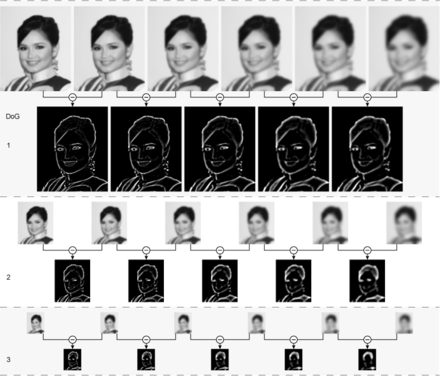
\includegraphics[scale=0.6]{DoG.png}
    \caption{Difference of Gaussians illustration (example from wikipedia)}\label{fig:Difference of Gaussians}
\end{figure}








\begin{figure}[h]
    \center
    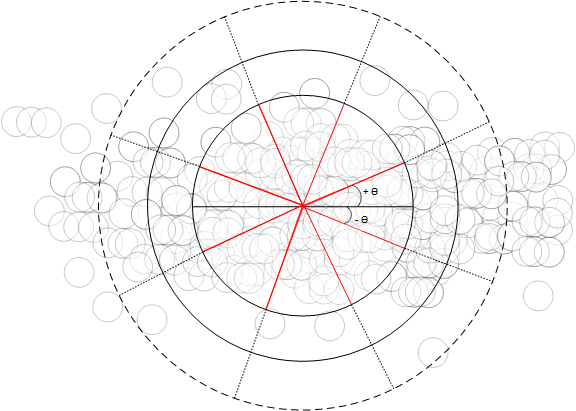
\includegraphics[scale=0.65]{QuantificationSpherique.png}
    \caption{Spheric quantizaton}\label{fig:Qantification sph�rique}
\end{figure}




% ----------------------------------------------------------------
\end{document} 